\section{Definition and Comparison to Stream Ciphers}

In symmetric cryptography, block ciphers and stream ciphers are two main types~\cite{Paar2024}.

Stream ciphers encrypt data one bit or one byte at a time. They use a \textit{keystream}, where each keystream bit is added to a plaintext bit individually~\cite{Paar2024}.

\begin{figure}[H]
    \centering
    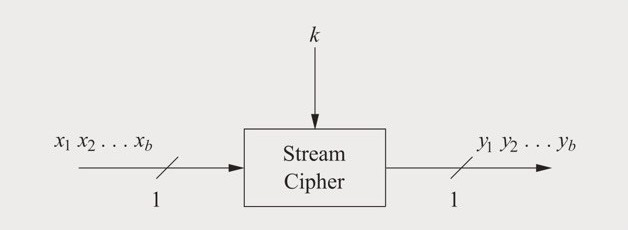
\includegraphics[width=0.7\textwidth]{streamc.jpeg}
    \caption{Stream cipher operation~\cite{Paar2024}.}
    \label{fig:stream_cipher}
\end{figure}

Block ciphers process fixed-size blocks of data, with each block encrypted separately~\cite{Paar2024}.

\begin{figure}[H]
    \centering
    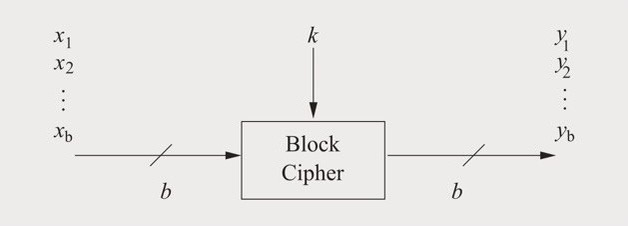
\includegraphics[width=0.7\textwidth]{blockc.jpeg}
    \caption{Block cipher operation~\cite{Paar2024}.}
    \label{fig:block_cipher}
\end{figure}

\begin{table}[H]
\centering
\begin{tabular}{|c|c|}
\hline
\textbf{Block Cipher} & \textbf{Stream Cipher} \\
\hline
Encrypts chunks (blocks) & Encrypts continuously, bit by bit \\
\hline
Offers more security when used properly & Can be faster and have less delay \\
\hline
\end{tabular}
\caption{Comparison between block cipher and stream cipher~\cite{Paar2024}.}
\label{tab:block_vs_stream}
\end{table}